\documentclass[10pt,a4paper,titlepage]{article}
\usepackage[utf8]{inputenc}
\usepackage{amsmath}
\usepackage{amsfonts}
\usepackage[T1]{fontenc}
\usepackage{graphicx}
\usepackage{csvsimple}
\usepackage{pdfpages}
\usepackage{float}
\usepackage[margin=2.5cm]{geometry}
\setlength{\parindent}{0in}
\author{Helen Harman \\ Student Number : 110007212 \\ Computer Science Department, Aberystwyth University}
\title{SE31520 Assignment : Enhancing the CS-Alumni Application}

\begin{document}

\maketitle

\tableofcontents

\pagebreak 
\section{Introduction}
\section{Architecture}
I have not changed the functionality of the CSA application, so see Loftus \cite[5]{design} for a class diagram for CSA.
\begin{figure}[H]
\begin{center}
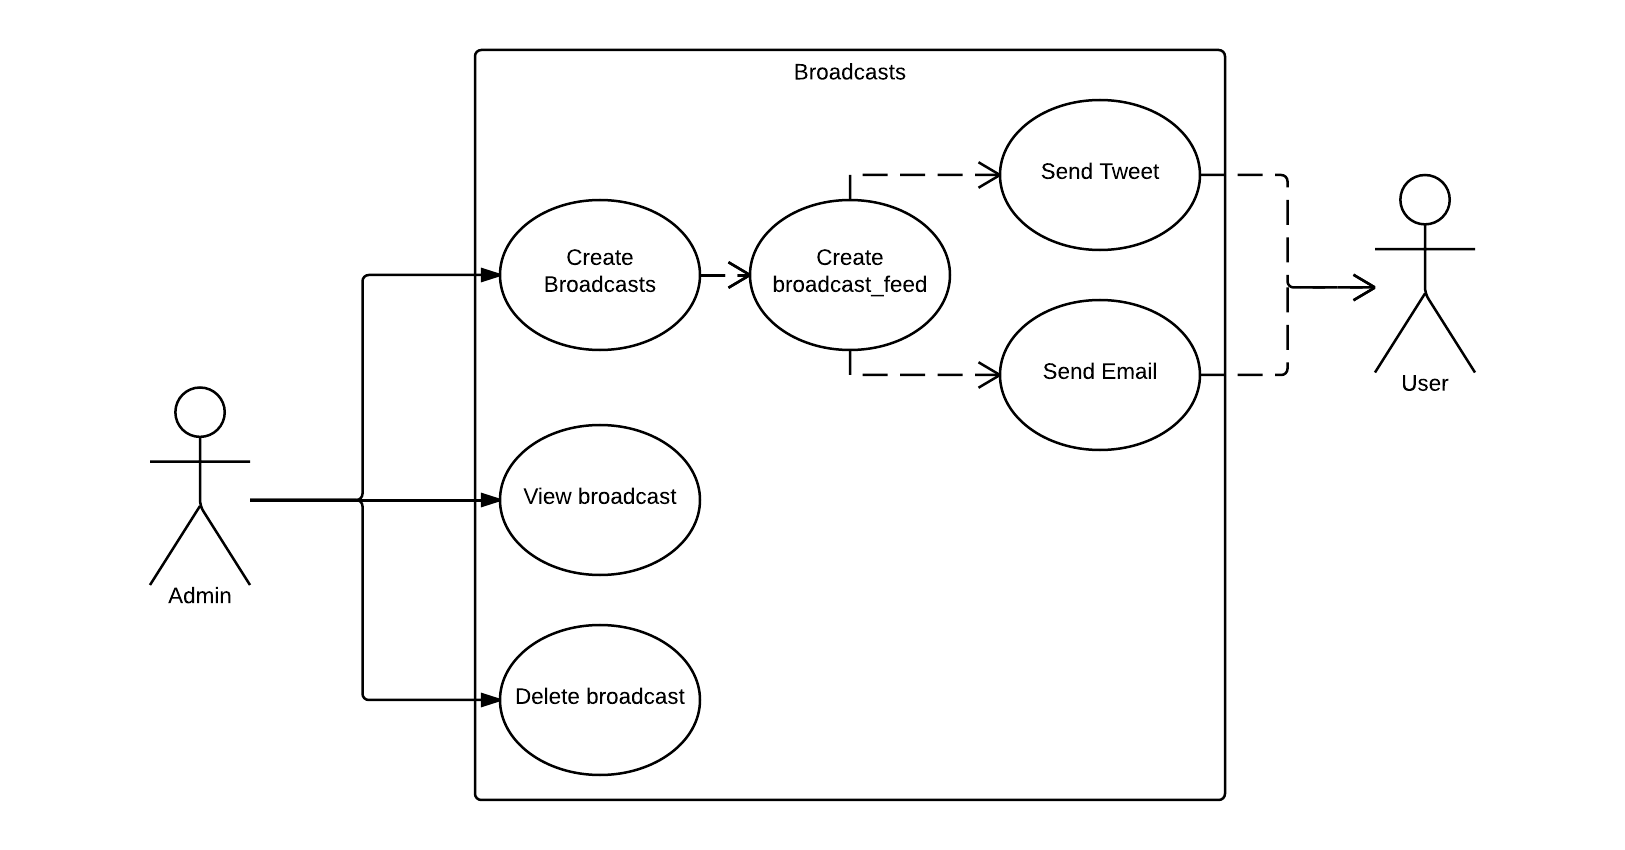
\includegraphics[scale=0.3]{include/broadcasts_Use_Case.png}  
\caption{Architecture : Use case for broadcasts. }
\label{fig:broadcastUseCase}
\end{center}
\end{figure}

\begin{figure}[H]
\begin{center}
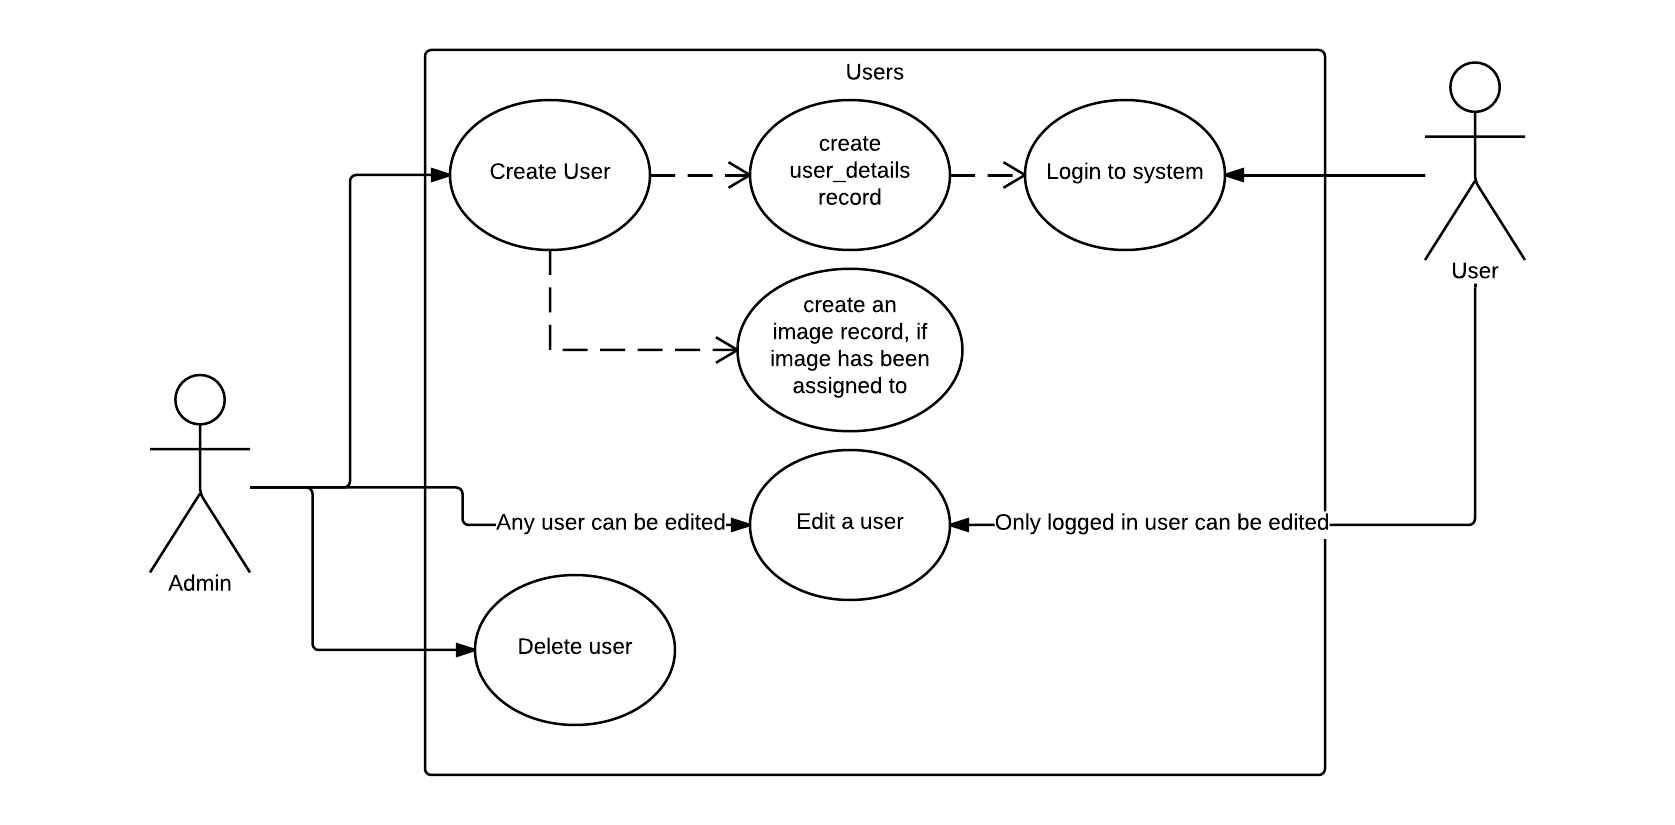
\includegraphics[scale=0.3]{include/User_Use_Case.png}  
\caption{Architecture : Use case for users. }
\label{fig:userUseCase}
\end{center}
\end{figure}


\begin{figure}[H]
\begin{center}
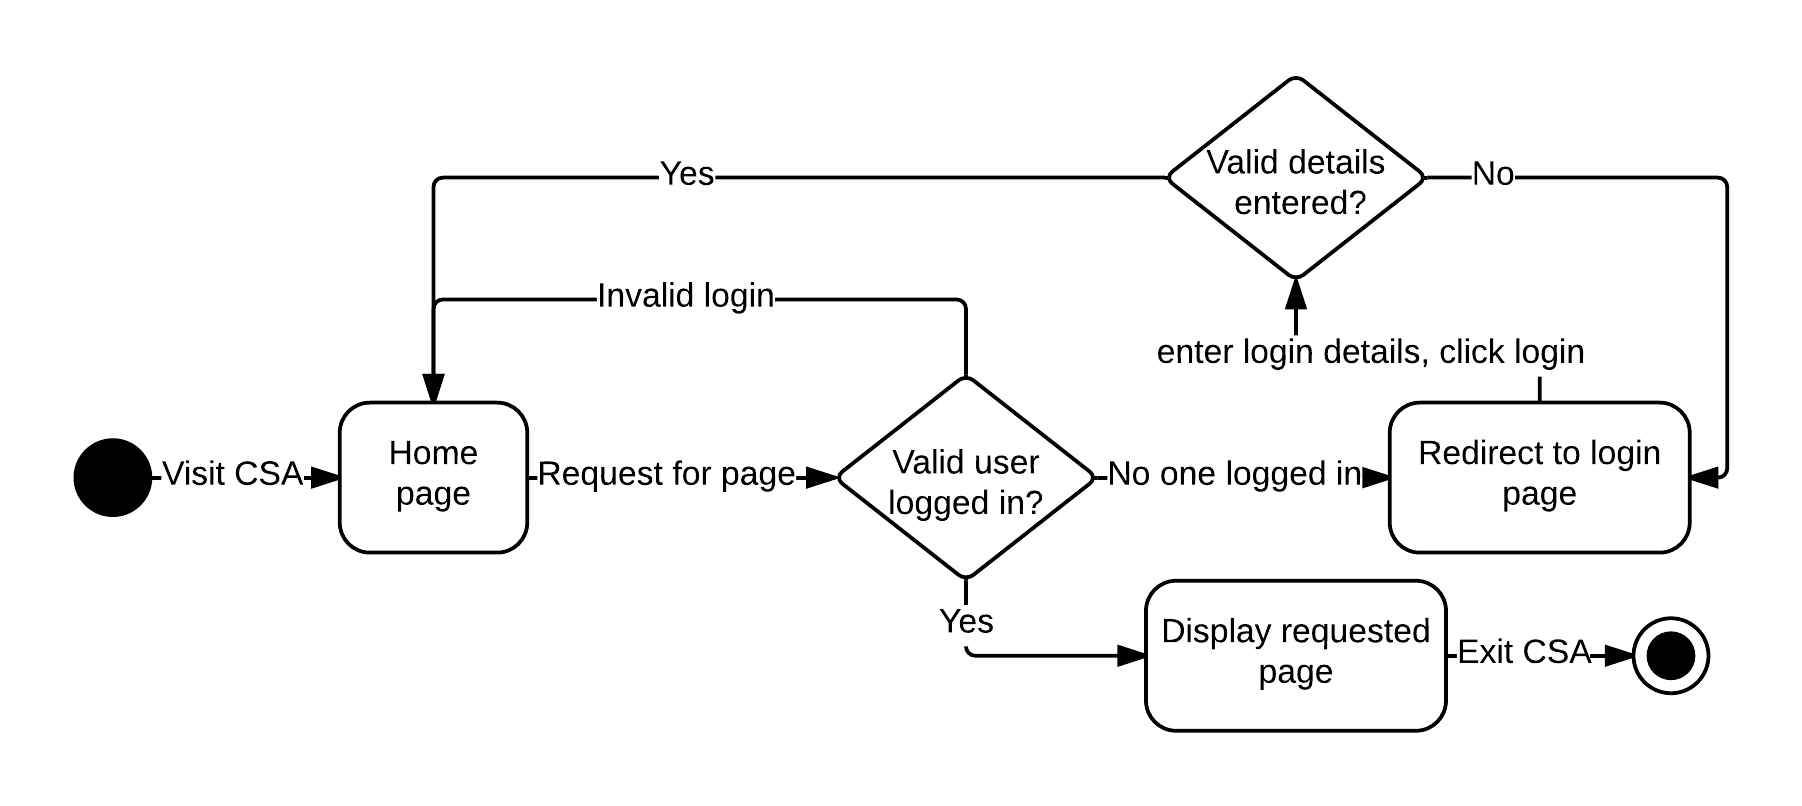
\includegraphics[scale=0.25]{include/State_Diagram.png}  
\caption{Architecture : State diagram. }
\label{fig:stateDiagram}
\end{center}
\end{figure}



\section{Test Strategy}
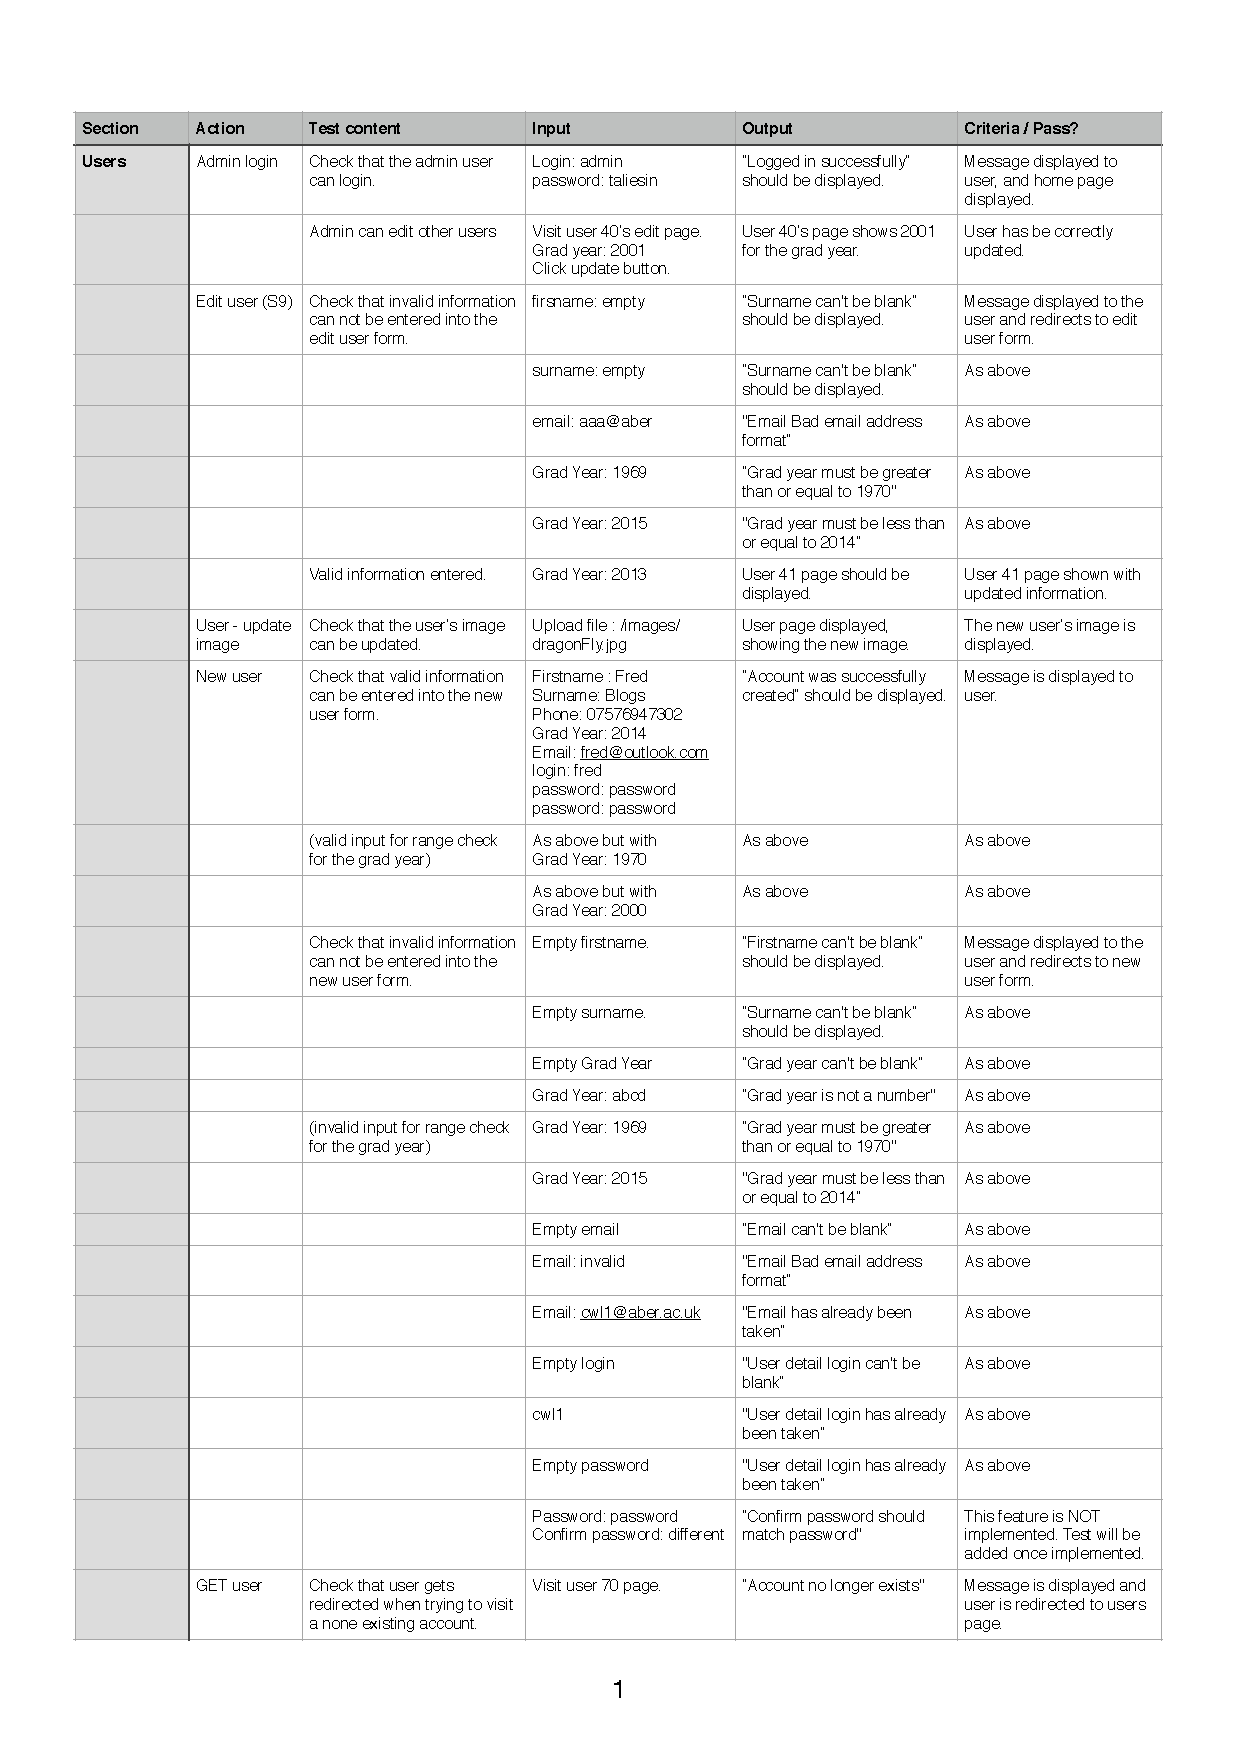
\includepdf[pages={1-3}]{include/testTable.pdf} 

\begin{figure}[H]
\begin{center}
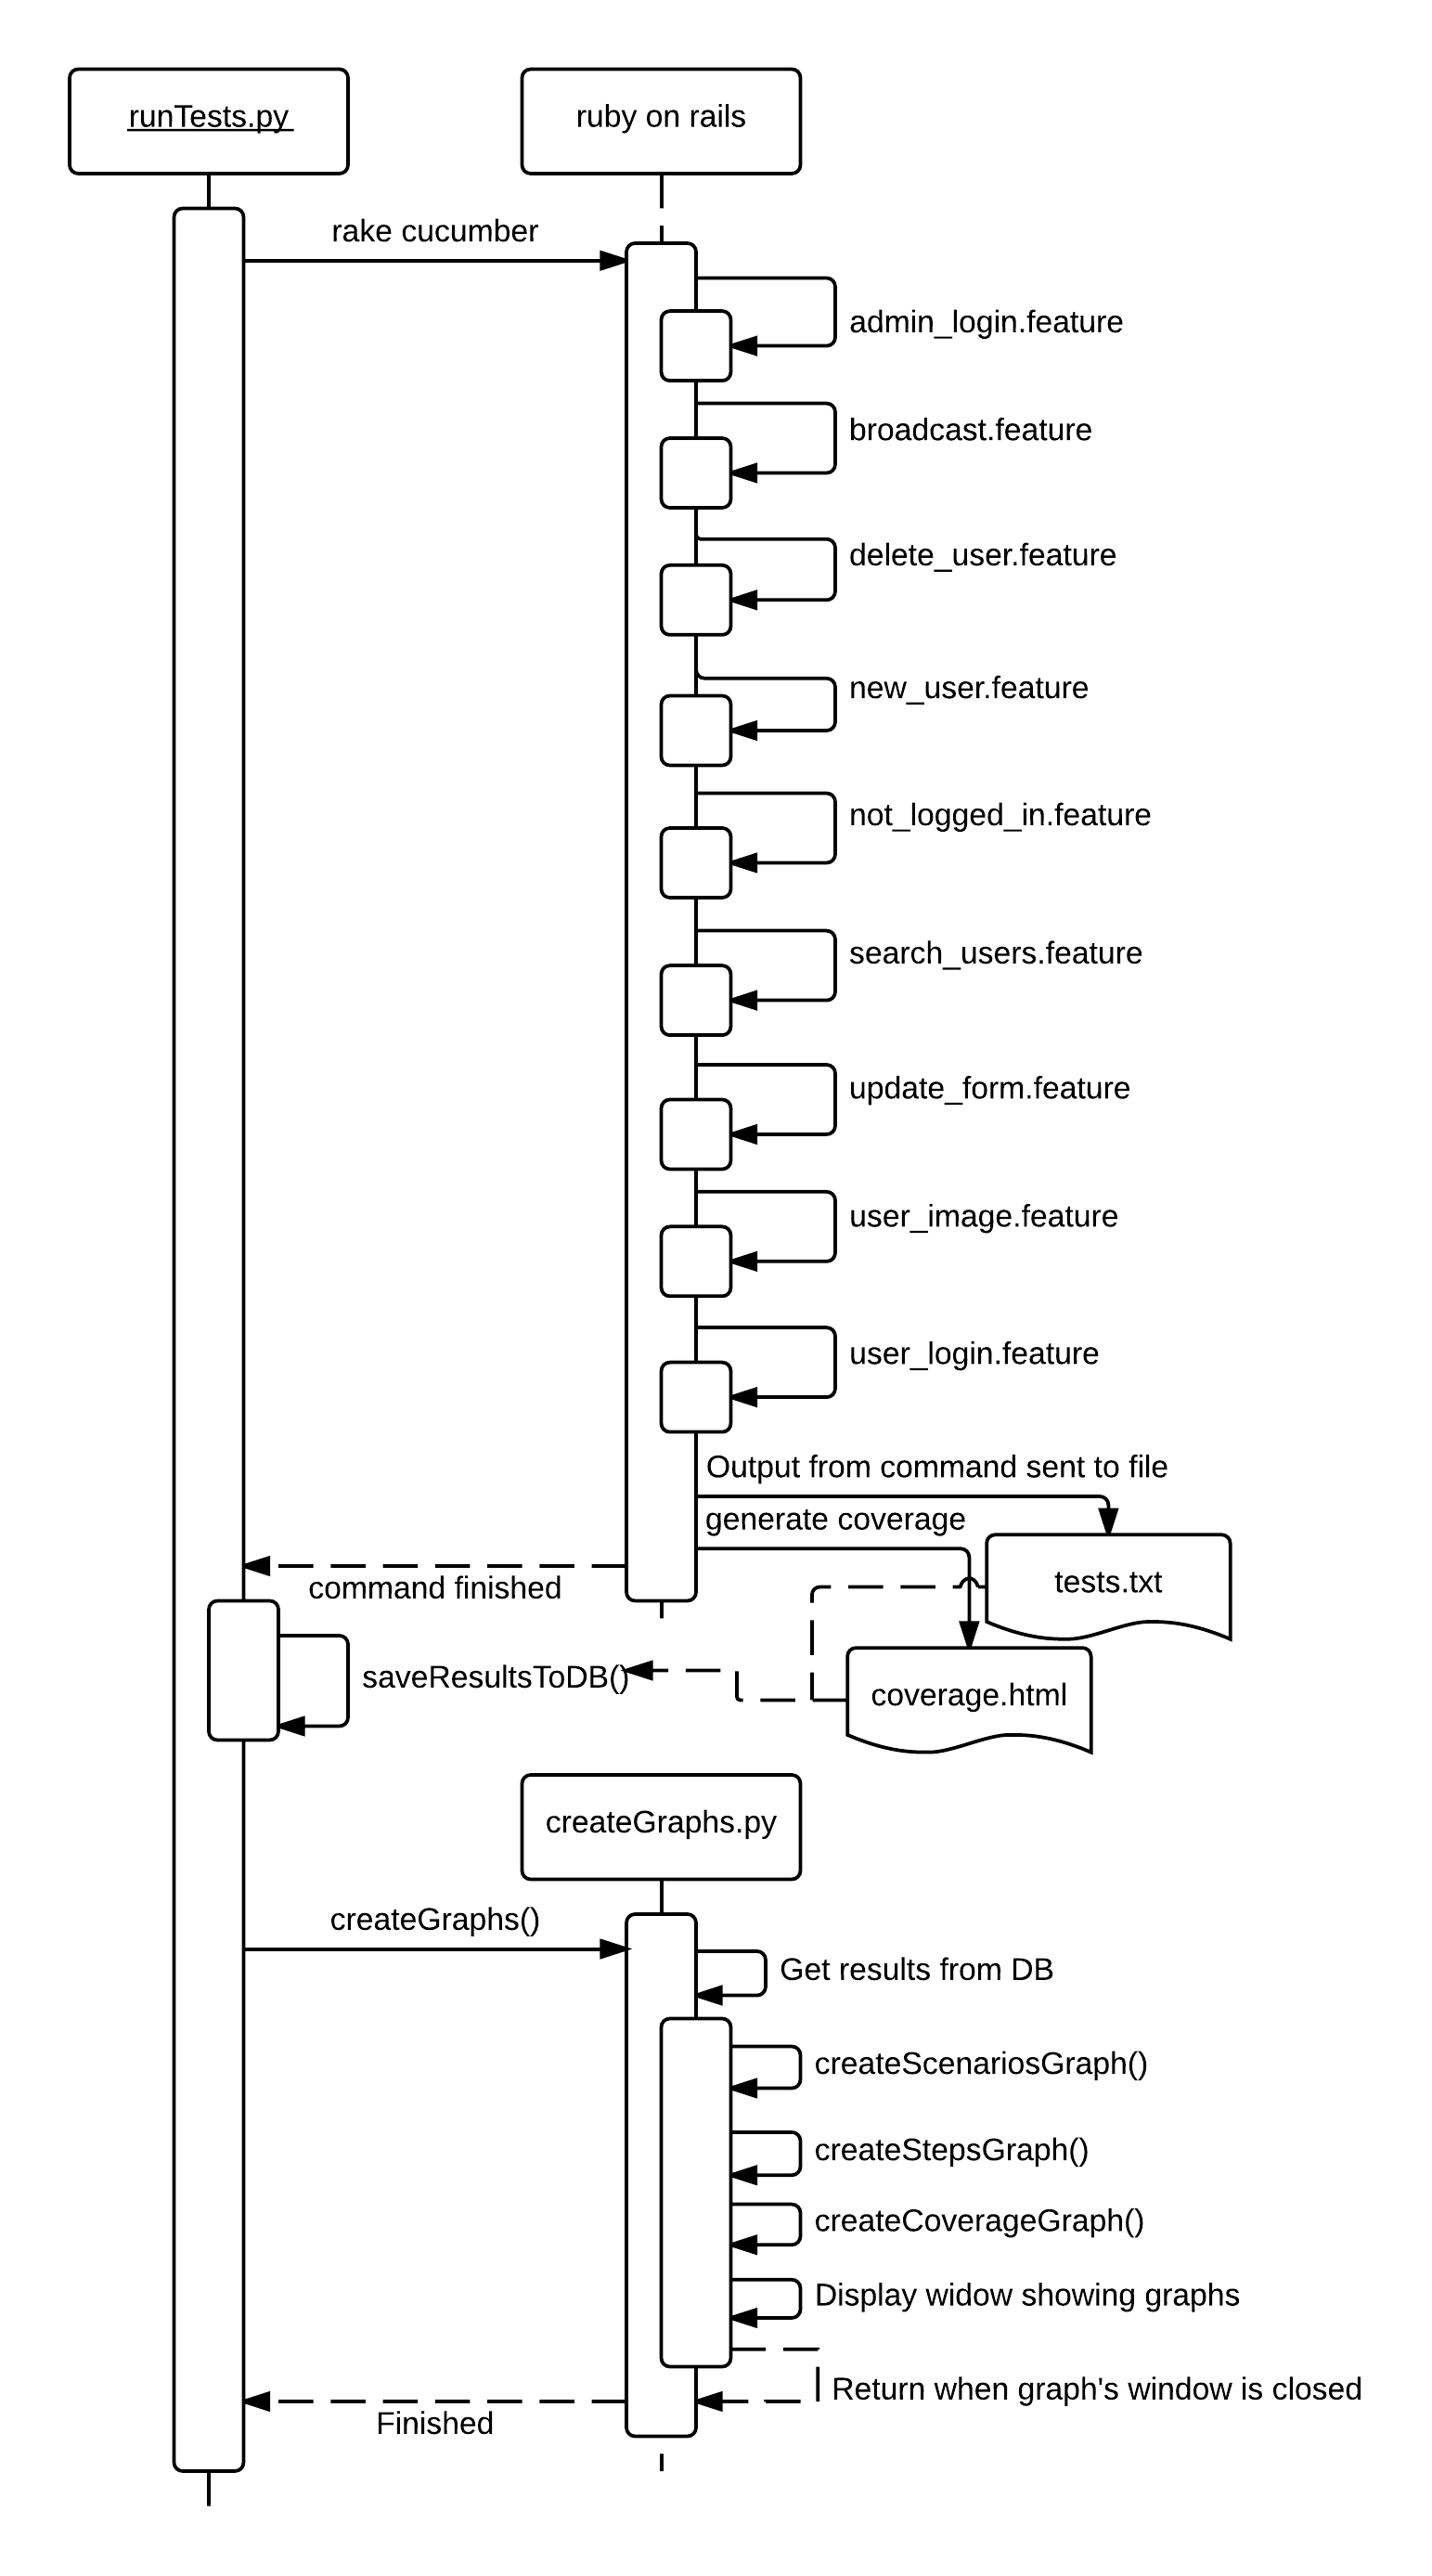
\includegraphics[scale=0.25]{include/Sequence_Diagram.png}  
\caption{Test Strategy : Sequence Diagram. }
\label{fig:stateDiagram}
\end{center}
\end{figure}

\section{Critical Evaluation}

\begin{thebibliography}{1}

\bibitem{design}Chris Loftus (2014), Requirements/Design for the CS-Alumni Application, [Online], Available: https://blackboard.aber.ac.uk/bbcswebdav/pid-487373-dt-content-rid-767088\_1/xid-767088\_1 [30 November 2014].

\end{thebibliography}

\end{document}